\documentclass[preview=true]{standalone}
\usepackage{tikz}
\usepackage{pgfplots}
\usepackage[siunitx, american]{circuitikz}
\usepackage[utf8]{inputenc}
\usepackage{newtxtext,newtxmath}
\usepackage[T1]{fontenc}
\pgfplotsset{compat=1.18}
\usepgfplotslibrary{units, fillbetween, smithchart, colormaps}
\usetikzlibrary{positioning, shapes, arrows, arrows.meta, graphs, shapes.geometric, math}
\tikzset{>=latex} % Better arrow tips

\begin{document}
    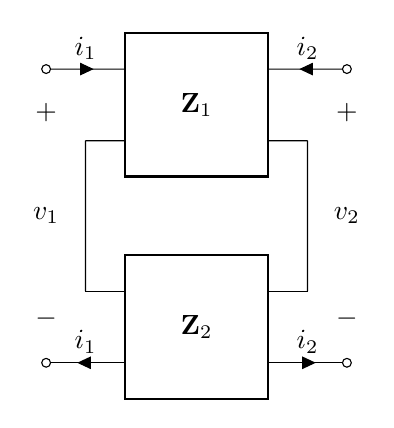
\begin{tikzpicture}
    \draw 
    node[fourport, t={$\mathbf{Z}_1$}, align=center] (z1) {} 
    (z1.port4) to[short, -o, ,i<_=$i_1$] ++(-1,0) coordinate (Z1A)
    (z1.port3) to[short, -o, ,i<=$i_2$] ++(1,0) coordinate (Z1B)
    (z1.port2) to[short] ++(0.5,0) coordinate (Z1C)
    (z1.port1) to[short] ++(-0.5,0) coordinate (Z1D)
    %(A) to[open, v=$v_1$,o-o] (D)
    %(B) to[open, v=$v_2$,o-o] (C)
    ;
    
    \draw 
    node[fourport, t={$\mathbf{Z}_2$}, below = of z1] (z2) {} 
    (z2.port4) to[short] ++(-0.5,0) coordinate (Z2A)
    (z2.port3) to[short] ++(0.5,0) coordinate (Z2B)
    (z2.port2) to[short, -o, i>=$i_2$] ++(1,0) coordinate (Z2C)
    (z2.port1) to[short, -o, i>_=$i_1$] ++(-1,0) coordinate (Z2D)
    %(A) to[open, v=$v_1$,o-o] (D)
    %(B) to[open, v=$v_2$,o-o] (C)
    ;

    \draw
    (Z1D) to[short] (Z2A)
    (Z1C) to[short] (Z2B)
    (Z1A) to[open, v=$v_1$] (Z2D)
    (Z1B) to[open, v=$v_2$] (Z2C)
    ;
    
    \end{tikzpicture}
\end{document}